\documentclass{article}

% content/resources/templates/preamble.tex
\usepackage[margin=0.6in]{geometry}
\author{Milav Dabgar}
\usepackage{amsmath,amssymb,amsthm}
\usepackage{booktabs}
\usepackage{multirow}
\usepackage{xcolor}
\usepackage{tcolorbox}
\tcbuselibrary{breakable,skins}
\usepackage[colorlinks=true,linkcolor=blue]{hyperref}
\usepackage{titlesec}
\usepackage{enumitem}
\usepackage{tikz}
\usepackage{pgfplots}
\usepackage{circuitikz}
\usepackage[version=4]{mhchem}
\usepackage{longtable}
\usepackage{array}
\usepackage{float}
\usepackage{caption}
\usepackage{listings}

\lstset{
  basicstyle=\small\ttfamily,
  breaklines=true,
  breakatwhitespace=false,
  postbreak=\mbox{\textcolor{red}{$\hookrightarrow$}\space},
  float=false,
  numbers=left,
  numberstyle=\tiny\color{gray},
  numbersep=10pt,
  xleftmargin=2em,
  keywordstyle=\color{blue},
  commentstyle=\color{green!60!black},
  stringstyle=\color{purple},
  backgroundcolor=\color{gray!5},
  showstringspaces=false,
  tabsize=2,
  captionpos=b,
  keepspaces=true,
  columns=flexible
}

\pgfplotsset{compat=1.18}
\usetikzlibrary{shapes,arrows,positioning,calc,patterns,decorations.pathmorphing,decorations.markings,arrows.meta}

% Color scheme
\definecolor{headcolor}{RGB}{0,102,204}
\definecolor{keycolor}{RGB}{220,20,60}
\definecolor{solutioncolor}{RGB}{34,139,34}
\definecolor{mnemoniccolor}{RGB}{148,0,211}
\definecolor{codecolor}{RGB}{0,0,100}

% Spacing
\setlength{\parskip}{3pt}
\setlist[itemize]{nosep}
\setlist[enumerate]{nosep}

% Title formatting
\titleformat{\section}{\Large\bfseries\color{headcolor}}{\thesection}{1em}{}
\titleformat{\subsection}{\large\bfseries\color{headcolor}}{\thesubsection}{1em}{}

% Pandoc tightlist compatibility
\providecommand{\tightlist}{%
  \setlength{\itemsep}{0pt}\setlength{\parskip}{0pt}}

% Pandoc longtable compatibility
\newcounter{none}
\def\thenone{}


% content/resources/templates/english-boxes.tex

% Custom environments
\newtcolorbox{solutionbox}{
 breakable,
 enhanced,
 colback=solutioncolor!5!white,
 colframe=solutioncolor!75!black,
 fonttitle=\bfseries,
 title=Solution
}

\newtcolorbox{solutionboxnobreak}{
 colback=solutioncolor!5!white,
 colframe=solutioncolor!75!black,
 fonttitle=\bfseries,
 title=Solution
}

\newtcolorbox{keyformula}{
 breakable,
 enhanced,
 colback=keycolor!5!white,
 colframe=keycolor!75!black,
 fonttitle=\bfseries,
 title=Key Formula
}

\newtcolorbox{mnemonicboxenv}{
 breakable,
 enhanced,
 colback=mnemoniccolor!5!white,
 colframe=mnemoniccolor!75!black,
 fonttitle=\bfseries,
 title=Mnemonic
}

\newcommand{\mnemonicbox}[1]{%
  \begin{mnemonicboxenv}
    #1
  \end{mnemonicboxenv}
}


% Custom commands for GTU solutions
% This file defines semantic commands for consistent formatting

% Question command with automatic formatting
\newcommand{\question}[2]{%
  \section*{Question #1}%
  \textbf{#2}%
}

% OR question variant
\newcommand{\questionor}[2]{%
  \section*{Question #1 OR}%
  \textbf{#2}%
}

% Proper table environment with caption
\newenvironment{answertable}[1]{%
  \begin{table}[htbp]
  \centering
  \caption{#1}
}{%
  \end{table}
}

% Proper figure environment for diagrams
\newenvironment{answerdiagram}[1]{%
  \begin{figure}[htbp]
  \centering
  \caption{#1}
}{%
  \end{figure}
}

% Semantic markup for key terms
\newcommand{\keyword}[1]{\textbf{#1}}
\newcommand{\code}[1]{\texttt{#1}}
\newcommand{\classname}[1]{\texttt{#1}}
\newcommand{\methodname}[1]{\texttt{#1}}

% Proper quotation marks
\newcommand{\mnemonic}[1]{``#1''}


\title{Linear Integrated Circuit (4341105) - Summer 2024 Solution}
\date{June 15, 2024}

\begin{document}
\maketitle
\solutiontitle

% Question 1(a) [3 marks]
\questionmarks{1}{a}{3}
\textbf{State and explain the difference between positive and negative feedback with diagram.}

\begin{solutionbox}
    \begin{tabulary}{\textwidth}{L|L|L}
        \toprule
        \textbf{Parameter} & \textbf{Negative Feedback} & \textbf{Positive Feedback} \\
        \midrule
        Signal & Output signal is fed back to input with opposite phase & Output signal is fed back to input with same phase \\
        Gain & Decreases & Increases \\
        Stability & Improves & Reduces \\
        Applications & Amplifiers & Oscillators \\
        \bottomrule
    \end{tabulary}
    \vspace{1em}

    \textbf{Diagram:}
    \begin{center}
    \begin{tikzpicture}[node distance=2cm, auto, >=latex]
        % Nodes
        \node [gtu input] (input) {Input};
        \node [gtu block, right of=input, node distance=2.5cm] (amp) {Amplifier};
        \node [gtu output, right of=amp, node distance=2.5cm] (output) {Output};
        \node [gtu block, below of=amp] (feedback) {Feedback Network};

        % Arrows
        \draw [gtu arrow] (input) -- (amp);
        \draw [gtu arrow] (amp) -- (output);
        \draw [gtu arrow] (output.south) |- (feedback.east);
        
        % Negative Feedback Loop
        \draw [gtu arrow] (feedback.west) -| node[near start] {Negative (-)} (amp.south);

        % Label for context 
        \node[below=1cm of feedback] {Feedback Diagram};
    \end{tikzpicture}
    \end{center}

    \begin{itemize}
        \item \textbf{Phase relationship}: In negative feedback, signal is 180$^\circ$ out of phase while in positive feedback, signal is in phase.
        \item \textbf{Purpose}: Negative feedback stabilizes system while positive feedback creates oscillations.
    \end{itemize}

    \begin{mnemonicbox}
        \mnemonic{Negative Needs Stability, Positive Produces Oscillations}
    \end{mnemonicbox}
\end{solutionbox}

% Question 1(b) [4 marks]
\questionmarks{1}{b}{4}
\textbf{Explain the effect of negative feedback on input impedance of the Amplifier.}

\begin{solutionbox}
    \begin{tabulary}{\textwidth}{L|L|L}
        \toprule
        \textbf{Type of Feedback} & \textbf{Effect on Input Impedance} & \textbf{Formula} \\
        \midrule
        Voltage Series & Increases & $Z_{in-f} = Z_{in}(1+A\beta)$ \\
        Current Series & Increases & $Z_{in-f} = Z_{in}(1+A\beta)$ \\
        Voltage Shunt & Decreases & $Z_{in-f} = Z_{in}/(1+A\beta)$ \\
        Current Shunt & Decreases & $Z_{in-f} = Z_{in}/(1+A\beta)$ \\
        \bottomrule
    \end{tabulary}
    \vspace{1em}

    \begin{itemize}
        \item \textbf{Series feedback}: When feedback signal is in series with input, input impedance increases.
        \item \textbf{Shunt feedback}: When feedback signal is in parallel with input, input impedance decreases.
        \item \textbf{Magnitude}: Change is proportional to $(1+A\beta)$ where $A$ is gain and $\beta$ is feedback factor.
    \end{itemize}

    \begin{mnemonicbox}
        \mnemonic{Series Soars, Shunt Shrinks}
    \end{mnemonicbox}
\end{solutionbox}

% Question 1(c) [7 marks]
\questionmarks{1}{c}{7}
\textbf{List the advantages and Disadvantages of negative feedback.}

\begin{solutionbox}
    \begin{tabulary}{\textwidth}{L|L}
        \toprule
        \textbf{Advantages} & \textbf{Disadvantages} \\
        \midrule
        Stabilizes gain & Reduces overall gain \\
        Increases bandwidth & Requires additional components \\
        Reduces distortion & May cause oscillation if improperly designed \\
        Reduces noise & Requires careful phase compensation \\
        Improves input/output impedance & Increases power consumption \\
        Reduces temperature sensitivity & Makes circuit more complex \\
        Controls frequency response & May reduce signal-to-noise ratio in some cases \\
        \bottomrule
    \end{tabulary}

    \begin{itemize}
        \item \textbf{Performance tradeoff}: Sacrifices gain to achieve better stability and linearity.
        \item \textbf{Frequency considerations}: May require compensation to prevent oscillations at high frequencies.
        \item \textbf{Design complexity}: More complex to design properly but offers better long-term performance.
    \end{itemize}

    \begin{mnemonicbox}
        \mnemonic{Stability Grows As Gain Drops}
    \end{mnemonicbox}
\end{solutionbox}

% Question 1(c) OR [7 marks]
\questionmarks{1}{c}{7}
\textbf{Explain Voltage series feedback amplifier in detail with block diagram and draw the Practical voltage series feedback circuit.}

\begin{solutionbox}
    \begin{tabulary}{\textwidth}{L|L}
        \toprule
        \textbf{Parameter} & \textbf{Effect in Voltage Series Feedback} \\
        \midrule
        Input signal & Voltage \\
        Feedback signal & Voltage \\
        Input impedance & Increases \\
        Output impedance & Decreases \\
        Gain stability & Improves \\
        Bandwidth & Increases \\
        \bottomrule
    \end{tabulary}
    \vspace{1em}

    \textbf{Block Diagram:}
    \begin{center}
    \begin{tikzpicture}[node distance=2cm, auto, >=latex]
        \node [gtu input] (gain) {Amplifier A};
        \node [gtu block, below of=gain] (feedback) {Feedback Network $\beta$};
        \node [left of=gain, node distance=2cm] (mix) {Mixer};
        \node [right of=gain, node distance=2cm] (sample) {Sampler};
        \node [gtu input, left of=mix] (input) {$V_{in}$};
        \node [gtu output, right of=sample] (output) {$V_{out}$};

        \draw [gtu arrow] (input) -- (mix);
        \draw [gtu arrow] (mix) -- (gain);
        \draw [gtu arrow] (gain) -- (sample);
        \draw [gtu arrow] (sample) -- (output);
        \draw [gtu arrow] (sample) |- (feedback);
        \draw [gtu arrow] (feedback) -| (mix);
    \end{tikzpicture}
    \end{center}

    \textbf{Practical Circuit:}
    \begin{center}
    \begin{circuitikz}[american voltages]
        \draw (0,0) node[npn](Q1){Q1}
        (Q1.E) to[R, l=$R_E$] (0,-2) node[ground]{}
        (Q1.C) to[short] (0,1) to[R, l=$R_C$] (0,3) node[vcc]{$+V_{CC}$}
        (Q1.B) to[short] (-1,0) to[C, l=$C_{in}$] (-2,0) node[left]{$V_{in}$}
        (0,1) to[short] (1,1) to[C, l=$C_{out}$] (2,1) node[right]{$V_{out}$}
        
        % Bias resistors
        (-1,0) to[R, l=$R_2$, *-] (-1,-2) node[ground]{}
        (-1,0) to[R, l=$R_1$, *-] (-1,3) to[short] (0,3);
    \end{circuitikz}
    \end{center}

    \begin{itemize}
        \item \textbf{Sampling method}: Output voltage is sampled and fed back to input.
        \item \textbf{Mixing method}: Feedback signal is mixed in series with input signal.
        \item \textbf{Working principle}: Reduces gain for improved stability and linearity.
        \item \textbf{Applications}: Audio amplifiers, instrumentation amplifiers.
    \end{itemize}
    
    \begin{mnemonicbox}
        \mnemonic{Voltage Series - Impedance In Up, Out Down}
    \end{mnemonicbox}
\end{solutionbox}

% Question 2(a) [3 marks]
\questionmarks{2}{a}{3}
\textbf{Write short note on Colpitts oscillator circuit.}

\begin{solutionbox}
    \begin{tabulary}{\textwidth}{L|L}
        \toprule
        \textbf{Component} & \textbf{Function} \\
        \midrule
        LC Tank & Determines oscillation frequency \\
        Capacitive Voltage Divider & Provides feedback \\
        Active Device & Provides gain to sustain oscillations \\
        \bottomrule
    \end{tabulary}
    \vspace{1em}

    \textbf{Circuit Diagram:}
    \begin{center}
    \begin{circuitikz}[american]
        \draw (0,0) node[npn](Q){Q}
        (Q.E) to[R, l=$R_E$] (0,-2) node[ground]{}
        (Q.C) to[L, l=$L_{RFC}$] (0,2) node[vcc]{$+V_{CC}$}
        (Q.C) to[C, l=$C_{out}$] (2,0) -- (2,-2)
        (2,0) to[short] (3,0) node[right]{Output}
        
        % Tank
        (4,0) to[L, l=$L$] (4,-2)
        (5,0) to[C, l=$C_1$] (5,-1) to[C, l=$C_2$] (5,-2)
        (5,-1) to[short] (4,-1) % Tap
        (2,-2) -- (5,-2) node[ground]{}
        
        % Feedback
        (5,-1) -- (5,-2.5) -- (-1,-2.5) -- (-1,0) to[short] (Q.B);
    \end{circuitikz}
    \end{center}

    \begin{itemize}
        \item \textbf{Frequency formula}: $f = \frac{1}{2\pi\sqrt{L \frac{C_1 C_2}{C_1 + C_2}}}$
        \item \textbf{Feedback}: Provided by capacitive voltage divider ($C_1$ and $C_2$).
        \item \textbf{Applications}: RF oscillators, communication circuits.
    \end{itemize}

    \begin{mnemonicbox}
        \mnemonic{Colpitts Contains Capacitive divider}
    \end{mnemonicbox}
\end{solutionbox}

% Question 2(b) [4 marks]
\questionmarks{2}{b}{4}
\textbf{Explain requirement of oscillator. i) Barkhausen Criterion. ii) Tank circuit. iii) Amplifier.}

\begin{solutionbox}
    \begin{tabulary}{\textwidth}{L|L|L}
        \toprule
        \textbf{Requirement} & \textbf{Function} & \textbf{Explanation} \\
        \midrule
        Barkhausen Criterion & Ensures sustained oscillation & Loop gain $A\beta = 1$, Phase shift = $0^\circ$ or $360^\circ$ \\
        Tank Circuit & Determines frequency & Resonant LC circuit that stores energy \\
        Amplifier & Provides gain & Compensates for circuit losses \\
        \bottomrule
    \end{tabulary}
    \vspace{1em}

    \textbf{Block Diagram:}
    \begin{center}
    \begin{tikzpicture}[node distance=2.5cm, auto, >=latex, every node/.style={align=center}]
        \node [gtu block] (amp) {Amplifier (A)};
        \node [gtu block, below of=amp] (feedback) {Feedback ($\beta$) \\ (Tank Circuit)};
        
        \draw [gtu arrow] (amp.east) -- ++(1,0) node[right] {Output} |- (feedback.east);
        \draw [gtu arrow] (feedback.west) -| (amp.west);
        
        \node [below of=feedback, node distance=1.5cm] {\textbf{Barkhausen Criterion}: $|A\beta| = 1, \angle A\beta = 0^\circ/360^\circ$};
    \end{tikzpicture}
    \end{center}

    \begin{itemize}
        \item \textbf{Barkhausen Criterion}: Mathematical condition for sustained oscillations without damping.
        \item \textbf{Tank Circuit}: LC circuit that determines frequency of oscillations.
        \item \textbf{Amplifier}: Active device that provides energy to maintain oscillations.
    \end{itemize}

    \begin{mnemonicbox}
        \mnemonic{BAT - Barkhausen Amplifies Tank}
    \end{mnemonicbox}
\end{solutionbox}

% Question 2(c) [7 marks]
\questionmarks{2}{c}{7}
\textbf{Explain construction, working and V-I characteristics of UJT.}

\begin{solutionbox}
    \begin{itemize}
        \item \textbf{Construction}: Silicon bar with two base connections ($B_1, B_2$) and one P-type emitter ($E$).
        \item \textbf{Symbol}: Triangle with emitter on one side pointing in.
        \item \textbf{Working}: When emitter voltage $V_E > \eta V_{BB}$, the PN junction becomes forward biased and $R_{B1}$ drops significantly (Negative Resistance).
        \item \textbf{Intrinsic Standoff Ratio ($\eta$)}: Ratio determining the triggering voltage.
    \end{itemize}

    \textbf{Symbol and Equivalent Circuit:}
    \begin{center}
    \begin{circuitikz}
        % Symbol
        \draw (0,0) node[ujt, xscale=1.5, yscale=1.5] (U) {};
        \node[above] at (U.B2) {B2};
        \node[below] at (U.B1) {B1};
        \node[left] at (U.E) {E};
        
        % Equivalent
        \draw (4,2) node[above]{B2} -- (4,1) to[R, l=$R_{B2}$] (4,0) -- (4,-1) to[R, l=$R_{B1}$] (4,-2) node[below]{B1};
        \draw (2,0) node[left]{E} to[D] (4,0);
    \end{circuitikz}
    \end{center}

    \textbf{V-I Characteristics:}
    \begin{center}
    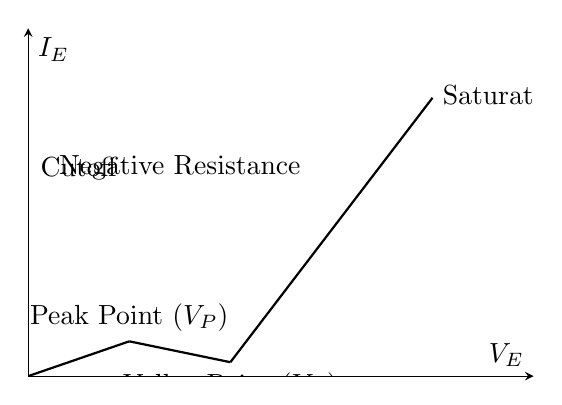
\begin{tikzpicture}
        \begin{axis}[
            width=8cm, height=6cm,
            axis lines=middle,
            xlabel=$V_E$, ylabel=$I_E$,
            xmin=0, xmax=5, ymin=0, ymax=5,
            xtick=\empty, ytick=\empty
        ]
            % Cutoff
            \draw[thick] (0,0) -- (1,0.5);
            % Negative resistance
            \draw[thick] (1,0.5) node[above]{Peak Point ($V_P$)} -- (2,0.2) node[below]{Valley Point ($V_V$)};
            % Saturation
            \draw[thick] (2,0.2) -- (4,4) node[right]{Saturation Region};
            
            \node at (0.5, 3) {Cutoff};
            \node at (1.5, 3) {Negative Resistance};
        \end{axis}
    \end{tikzpicture}
    \end{center}

    \begin{mnemonicbox}
        \mnemonic{UJT Peaks Then Valleys - Negative Resistance Rules}
    \end{mnemonicbox}
\end{solutionbox}

% Question 2(a) OR [3 marks]
\questionmarks{2}{a}{3}
\textbf{State the advantages, disadvantages and applications of Hartley oscillator.}

\begin{solutionbox}
    \begin{tabulary}{\textwidth}{L|L|L}
        \toprule
        \textbf{Advantages} & \textbf{Disadvantages} & \textbf{Applications} \\
        \midrule
        Easy tuning & Bulky inductors & RF generators \\
        Wide frequency range & Mutual inductance issues & Radio receivers \\
        Simple design & Difficult at high frequencies & Amateur radio \\
        Good frequency stability & Requires center-tapped coil & Communication equipment \\
        \bottomrule
    \end{tabulary}
    \vspace{1em}

    \textbf{Circuit Diagram:}
    \begin{center}
    \begin{circuitikz}[american]
        \draw (0,0) node[npn](Q){Q}
        (Q.E) to[R, l=$R_E$] (0,-2) node[ground]{}
        (Q.C) to[L, l=$L_{RFC}$] (0,2) node[vcc]{$+V_{CC}$}
        (Q.C) to[C, l=$C_{out}$] (2,0) -- (2,-2)
        
        % Tank
        (4,0) to[C, l=$C$] (4,-2)
        (5,0) to[L, l=$L_1$] (5,-1) to[L, l=$L_2$] (5,-2)
        (5,-1) to[short] (4,-1) % Tap
        (2,-2) -- (5,-2) node[ground]{}
        
        % Feedback
        (5,-1) -- (5,-2.5) -- (-1,-2.5) -- (-1,0) to[short] (Q.B);
    \end{circuitikz}
    \end{center}

    \begin{itemize}
        \item \textbf{Frequency}: $f = \frac{1}{2\pi\sqrt{(L_1+L_2)C}}$
        \item \textbf{Feature}: Split inductor tank circuit.
    \end{itemize}

    \begin{mnemonicbox}
        \mnemonic{Hartley Has tapped Inductor}
    \end{mnemonicbox}
\end{solutionbox}

% Question 2(b) OR [4 marks]
\questionmarks{2}{b}{4}
\textbf{Explain UJT as relaxation oscillator.}

\begin{solutionbox}
    \begin{tabulary}{\textwidth}{L|L}
        \toprule
        \textbf{Component} & \textbf{Function} \\
        \midrule
        UJT & Provides switching action \\
        Capacitor & Timing element \\
        Resistor & Controls charging rate \\
        Output & Sawtooth waveform \\
        \bottomrule
    \end{tabulary}
    \vspace{1em}

    \textbf{Circuit Diagram:}
    \begin{center}
    \begin{circuitikz}
        \draw (0,0) -- (4,0) node[ground]{}; % Ground rail
        \draw (0,4) -- (4,4) node[vcc]{$+V_{CC}$}; % Vcc rail
        
        \draw (1,4) to[R, l=$R$] (1,2) to[C, l=$C$] (1,0);
        \draw (3,2) node[ujt](U){};
        \draw (3,4) to[R, l=$R_2$] (U.B2);
        \draw (3,0) to[R, l=$R_1$] (U.B1);
        \draw (1,2) -- (U.E);
        
        \draw (U.B1) -- ++(1,0) node[right]{Pulse Out};
        \draw (1,2) -- (0,2) node[left]{Sawtooth Out};
    \end{circuitikz}
    \end{center}

    \begin{itemize}
        \item \textbf{Operation}: Capacitor charges via $R$ until $V_P$. UJT turns on, discharging C via $R_1$.
        \item \textbf{Frequency}: $f \approx \frac{1}{RC \ln(1/1-\eta)}$
    \end{itemize}

    \begin{mnemonicbox}
        \mnemonic{Charge-Fire-Repeat - Sawtooth's Beat}
    \end{mnemonicbox}
\end{solutionbox}

% Question 2(c) OR [7 marks]
\questionmarks{2}{c}{7}
\textbf{Explain working of weinbridge oscillator with neat diagram also state the advantage, disadvantage and application for the same.}

\begin{solutionbox}
    \begin{itemize}
        \item \textbf{Configuration}: Uses RC bridge network for feedback. Non-inverting amplifier.
        \item \textbf{Conditions}: $f = \frac{1}{2\pi RC}$, Gain $A \ge 3$.
        \item \textbf{Phase}: Net phase shift is $0^\circ$.
    \end{itemize}

    \textbf{Circuit Diagram:}
    \begin{center}
    \begin{circuitikz}[american]
        \draw (0,0) node[op amp](opamp){}
        (opamp.+) -- (-2, -0.5) to[C, l=$C$] (-2, -1.5) to[R, l=$R$] (-2, -2.5) node[ground]{}
        (-2, -0.5) to[R, l=$R$] (-2, 1) to[C, l=$C$] (0, 1) -- (opamp.-)
        (opamp.-) to[R, l=$R_1$] (-1, 0.5) node[ground]{}
        (opamp.out) -- (1,0) node[right]{$V_{out}$}
        (opamp.out) to[R, l=$R_f$] (0, 1.5) -- (0, 1) % Feedback
        (opamp.out) -- (0.5, 0) -- (0.5, -3) -- (-2, -2.5); % Feedback path to bridge
    \end{circuitikz}
    \end{center}

    \begin{tabulary}{\textwidth}{L|L}
        \toprule
        \textbf{Advantages} & \textbf{Disadvantages} \\
        \midrule
        High frequency stability & Limited frequency range \\
        Low distortion output & Amplitude stabilization needed \\
        Simple RC components & Sensitive to component variations \\
        Easy to tune & Difficult to start oscillations \\
        \bottomrule
    \end{tabulary}

    \begin{itemize}
        \item \textbf{Applications}: Audio signal generators, musical instruments.
    \end{itemize}

    \begin{mnemonicbox}
        \mnemonic{Wien Works at R1C1=R2C2 frequency}
    \end{mnemonicbox}
\end{solutionbox}

% Question 3(a) [3 marks]
\questionmarks{3}{a}{3}
\textbf{Give classification of power Amplifier.}

\begin{solutionbox}
    \begin{tabulary}{\textwidth}{L|L}
        \toprule
        \textbf{Classification Basis} & \textbf{Types} \\
        \midrule
        Conduction Angle & Class A ($360^\circ$), B ($180^\circ$), AB ($180^\circ$-$360^\circ$), C ($<180^\circ$) \\
        Configuration & Single-ended, Push-pull, Complementary \\
        Coupling & RC coupled, Transformer coupled, Direct coupled \\
        \bottomrule
    \end{tabulary}

    \begin{itemize}
        \item \textbf{Class A}: Highest linearity, lowest efficiency.
        \item \textbf{Class B}: Push-pull, crossover distortion.
        \item \textbf{Class C}: Tuned loads, highest efficiency.
    \end{itemize}

    \begin{mnemonicbox}
        \mnemonic{A All-time, B Bisects, AB Almost-Bisects, C Cuts-more}
    \end{mnemonicbox}
\end{solutionbox}

% Question 3(b) [4 marks]
\questionmarks{3}{b}{4}
\textbf{Explain class A power amplifier.}

\begin{solutionbox}
    \begin{tabulary}{\textwidth}{L|L}
        \toprule
        \textbf{Parameter} & \textbf{Class A Amplifier} \\
        \midrule
        Conduction Angle & $360^\circ$ (full cycle) \\
        Q-point & Center of load line \\
        Efficiency & Low (25-30\% practical, 50\% max theoretical) \\
        Distortion & Very low (High Fidelity) \\
        \bottomrule
    \end{tabulary}
    \vspace{1em}

    \textbf{Load Line Diagram:}
    \begin{center}
    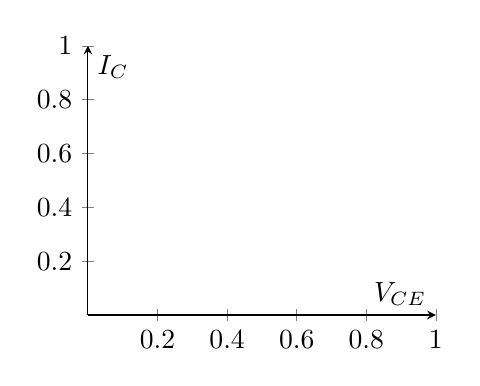
\begin{tikzpicture}
        \begin{axis}[
            width=6cm, height=5cm,
            axis lines=middle,
            xlabel=$V_{CE}$, ylabel=$I_C$,
            xtick=\empty, ytick=\empty
        ]
            \draw[thick] (0,4) -- (4,0); % Load line
            \node[circle, fill, inner sep=1.5pt, label=right:Q] at (2,2) {}; % Q point
            \node at (2.5, 3) {Load Line};
        \end{axis}
    \end{tikzpicture}
    \end{center}

    \begin{mnemonicbox}
        \mnemonic{Class A - Always conducting, All cycle}
    \end{mnemonicbox}
\end{solutionbox}

% Question 3(c) [7 marks]
\questionmarks{3}{c}{7}
\textbf{Explain the principle of push pull amplifiers and write short note on class B push pull amplifier.}

\begin{solutionbox}
    \begin{itemize}
        \item \textbf{Principle}: Uses two active devices driven in antiphase. One pushes current into load, other pulls current from load.
        \item \textbf{Class B Push-Pull}: Biased at cutoff. Transistor 1 conducts for positive half, Transistor 2 for negative half.
    \end{itemize}

    \textbf{Block Diagram:}
    \begin{center}
    \begin{tikzpicture}[node distance=2cm]
        \node [gtu input] (in) {Input};
        \node [gtu block, right of=in] (split) {Phase Splitter};
        \node [gtu block, right of=split, yshift=1cm] (Q1) {Q1 (NPN)};
        \node [gtu block, right of=split, yshift=-1cm] (Q2) {Q2 (PNP)};
        \node [gtu output, right of=split, xshift=3cm] (out) {Output};

        \draw [gtu arrow] (in) -- (split);
        \draw [gtu arrow] (split) |- (Q1);
        \draw [gtu arrow] (split) |- (Q2);
        \draw [gtu arrow] (Q1) -| (out);
        \draw [gtu arrow] (Q2) -| (out);
    \end{tikzpicture}
    \end{center}

    \textbf{Advantages and Disadvantages:}
    \begin{itemize}
        \item \textbf{Efficiency}: High (~78.5\%).
        \item \textbf{Harmonics}: Even harmonics cancel out.
        \item \textbf{Issue}: Crossover distortion due to $V_{BE}$ drop.
    \end{itemize}

    \begin{mnemonicbox}
        \mnemonic{Push-Pull: Pair Processes alternate Pulses}
    \end{mnemonicbox}
\end{solutionbox}

% Question 3(a) OR [3 marks]
\questionmarks{3}{a}{3}
\textbf{Discuss crossover distortion in push pull amplifier. How it can be removed.}

\begin{solutionbox}
    \begin{itemize}
        \item \textbf{Problem}: Power transistors in Class B need $\approx 0.7V$ to turn on. Input signal between -0.7V and +0.7V is not amplified, creating a dead zone.
        \item \textbf{Effect}: Distortion at the zero-crossing of the waveform.
    \end{itemize}

    \textbf{Waveform:}
    \begin{center}
    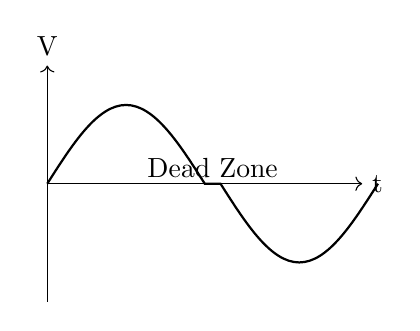
\begin{tikzpicture}
        \draw[->] (0,0) -- (4,0) node[right]{t};
        \draw[->] (0,-1.5) -- (0,1.5) node[above]{V};
        \draw[thick] (0,0) sin (1,1) cos (2,0) -- (2.2,0) sin (3.2,-1) cos (4.2,0);
        \node at (2.1, 0.2) {Dead Zone};
    \end{tikzpicture}
    \end{center}

    \begin{itemize}
        \item \textbf{Removal}: Use Class AB operation. Pre-bias the transistors using diodes or resistors so they are on the verge of conduction even with zero input.
    \end{itemize}

    \begin{mnemonicbox}
        \mnemonic{Cross to Class AB Smooths the Gap}
    \end{mnemonicbox}
\end{solutionbox}

% Question 3(b) OR [4 marks]
\questionmarks{3}{b}{4}
\textbf{Explain complimentary symmetry push-pull amplifier.}

\begin{solutionbox}
    \begin{itemize}
        \item \textbf{Concept}: Uses matched pair of NPN and PNP transistors.
        \item \textbf{Operation}: NPN conducts for positive half, PNP for negative half.
        \item \textbf{Advantage}: No phase splitter transformer needed.
    \end{itemize}

    \textbf{Circuit:}
    \begin{center}
    \begin{circuitikz}
        \draw (0,2) node[vcc]{$+V_{CC}$} to[short] (0,1) node[npn](Q1){Q1};
        \draw (0,-2) node[ground]{} to[short] (0,-1) node[pnp, anchor=C](Q2){Q2};
        \draw (Q1.E) -- (Q2.E);
        \draw (Q1.B) -- (Q2.B) to[short] (-1,0) node[left]{Input};
        \draw (0,0) to[C] (2,0) to[R, l=$R_L$] (2,-2) node[ground]{};
    \end{circuitikz}
    \end{center}

    \begin{mnemonicbox}
        \mnemonic{NPN Pulls-up, PNP Pulls-down}
    \end{mnemonicbox}
\end{solutionbox}

% Question 3(c) OR [7 marks]
\questionmarks{3}{c}{7}
\textbf{Derive the equation of efficiency for class B push pull Amplifier.}

\begin{solutionbox}
    \begin{itemize}
        \item \textbf{Input Power ($P_{DC}$)}:
        Total current from supply $I_{dc} = \frac{2I_m}{\pi}$.
        $$ P_{DC} = V_{CC} \times I_{dc} = \frac{2 V_{CC} I_m}{\pi} $$
        
        \item \textbf{Output Power ($P_{AC}$)}:
        RMS values $V_{rms} = \frac{V_m}{\sqrt{2}}$, $I_{rms} = \frac{I_m}{\sqrt{2}}$.
        $$ P_{AC} = V_{rms} I_{rms} = \frac{V_m I_m}{2} $$
        
        \item \textbf{Efficiency ($\eta$)}:
        $$ \eta = \frac{P_{AC}}{P_{DC}} \times 100\% $$
        $$ \eta = \frac{V_m I_m / 2}{2 V_{CC} I_m / \pi} \times 100\% = \frac{\pi}{4} \frac{V_m}{V_{CC}} \times 100\% $$
        
        \item \textbf{Maximum Efficiency}: When $V_m = V_{CC}$,
        $$ \eta_{max} = \frac{\pi}{4} \times 100\% \approx 78.5\% $$
    \end{itemize}

    \begin{mnemonicbox}
        \mnemonic{Pi-over-4 gives 78.5\% - Class B's best}
    \end{mnemonicbox}
\end{solutionbox}

% Question 4(a) [3 marks]
\questionmarks{4}{a}{3}
\textbf{Define.(i) CMRR (ii)slew rate.(iii)Input offset Current.}

\begin{solutionbox}
    \begin{tabulary}{\textwidth}{L|L|L}
        \toprule
        \textbf{Parameter} & \textbf{Definition} & \textbf{Typical} \\
        \midrule
        CMRR & Ratio of differential gain to common-mode gain ($A_d/A_{cm}$). Rejection capability. & 90 dB \\
        Slew Rate & Max rate of change of output voltage ($dV_o/dt$). Speed of response. & 0.5 V/$\mu$s \\
        Input Offset Current & Difference between base currents ($|I_{B1} - I_{B2}|$). & 20-200 nA \\
        \bottomrule
    \end{tabulary}

    \begin{mnemonicbox}
        \mnemonic{Cancelling Mistakes Requires Ratios}
    \end{mnemonicbox}
\end{solutionbox}

% Question 4(b) [4 marks]
\questionmarks{4}{b}{4}
\textbf{Draw and explain the basic block diagram of an operational amplifier.}

\begin{solutionbox}
    \begin{center}
    \begin{tikzpicture}[node distance=2.5cm, auto, >=latex]
        \node [gtu input] (in) {Inputs};
        \node [gtu block, right of=in] (diff) {Differential\\Amplifier};
        \node [gtu block, right of=diff] (gain) {High Gain\\Stage};
        \node [gtu block, right of=gain] (level) {Level\\Shifter};
        \node [gtu block, right of=level] (outstage) {Output\\Stage};
        \node [right of=outstage, node distance=2cm] (out) {Output};

        \draw [gtu arrow] (in) -- (diff);
        \draw [gtu arrow] (diff) -- (gain);
        \draw [gtu arrow] (gain) -- (level);
        \draw [gtu arrow] (level) -- (outstage);
        \draw [gtu arrow] (outstage) -- (out);
    \end{tikzpicture}
    \end{center}

    \begin{itemize}
        \item \textbf{Differential Amp}: High input impedance, noise rejection.
        \item \textbf{High Gain}: Provides most voltage gain.
        \item \textbf{Level Shifter}: Resets DC level to zero.
        \item \textbf{Output Stage}: Low output impedance, current drive.
    \end{itemize}

    \begin{mnemonicbox}
        \mnemonic{Diff-Amp Gain Shift Out}
    \end{mnemonicbox}
\end{solutionbox}

% Question 4(c) [7 marks]
\questionmarks{4}{c}{7}
\textbf{Explain in detail operational amplifier as integrator.}

\begin{solutionbox}
    \begin{itemize}
        \item \textbf{Function}: Output is time integral of input.
        \item \textbf{Equation}: $V_{out} = -\frac{1}{RC} \int V_{in} dt$.
        \item \textbf{Components}: Resistor in input, Capacitor in feedback.
    \end{itemize}

    \textbf{Circuit Diagram:}
    \begin{center}
    \begin{circuitikz}[american]
        \draw (0,0) node[op amp](opamp){}
        (opamp.-) to[R, l=$R$] (-2, 0.5) node[left]{$V_{in}$}
        (opamp.+) node[ground]{}
        (opamp.-) -- (0, 0.5) -- (0, 1.5) to[C, l=$C$] (2, 1.5) -- (opamp.out)
        (opamp.out) -- (3,0) node[right]{$V_{out}$};
    \end{circuitikz}
    \end{center}

    \textbf{Waveforms:} Square wave input $\rightarrow$ Triangular wave output.

    \begin{mnemonicbox}
        \mnemonic{Square-In Triangle-Out, RC sets the Slope}
    \end{mnemonicbox}
\end{solutionbox}

% Question 4(a) OR [3 marks]
\questionmarks{4}{a}{3}
\textbf{Explain operational amplifier as summing amplifier.}

\begin{solutionbox}
    \begin{itemize}
        \item \textbf{Function}: Adds multiple input voltages.
        \item \textbf{Equation}: $V_{out} = -(\frac{R_f}{R_1}V_1 + \frac{R_f}{R_2}V_2 + \dots)$.
    \end{itemize}

    \textbf{Circuit:}
    \begin{center}
    \begin{circuitikz}[american]
        \draw (0,0) node[op amp](opamp){}
        (opamp.+) node[ground]{}
        (opamp.-) -- (-1, 0.5)
        (-1, 0.5) to[R, l=$R_1$] (-3, 1.5) node[left]{$V_1$}
        (-1, 0.5) to[R, l=$R_2$] (-3, 0.5) node[left]{$V_2$}
        (opamp.-) -- (0, 0.5) -- (0, 1.5) to[R, l=$R_f$] (2, 1.5) -- (opamp.out)
        (opamp.out) -- (3,0) node[right]{$V_{out}$};
    \end{circuitikz}
    \end{center}

    \begin{mnemonicbox}
        \mnemonic{Many Inputs, One Output - Sum It All}
    \end{mnemonicbox}
\end{solutionbox}

% Question 4(b) OR [4 marks]
\questionmarks{4}{b}{4}
\textbf{State the applications of operational amplifier.}

\begin{solutionbox}
    \begin{itemize}
        \item \textbf{Linear}: Adder, Subtractor, Integrator, Differentiator, Instrumentation Amp.
        \item \textbf{Non-Linear}: Comparator, Schmitt Trigger, Rectifiers, Log amplifiers.
        \item \textbf{Waveform Generation}: Oscillators, Multivibrators.
        \item \textbf{Active Filters}: Low pass, High pass, Band pass filters.
    \end{itemize}

    \begin{mnemonicbox}
        \mnemonic{SMWIG-CR: Signal, Math, Wave, Instrument, Gate, Convert, Regulate}
    \end{mnemonicbox}
\end{solutionbox}

% Question 4(c) OR [7 marks]
\questionmarks{4}{c}{7}
\textbf{Explain op-amp as inverting and non-inverting amplifier.}

\begin{solutionbox}
    \begin{tabulary}{\textwidth}{L|L}
        \toprule
        \textbf{Inverting Amplifier} & \textbf{Non-Inverting Amplifier} \\
        \midrule
        Input at inverting terminal (-) & Input at non-inverting terminal (+) \\
        Phase shift $180^\circ$ & Phase shift $0^\circ$ \\
        Gain $A_v = -R_f/R_1$ & Gain $A_v = 1 + R_f/R_1$ \\
        Input Impedance $\approx R_1$ & Input Impedance $\approx \infty$ \\
        \bottomrule
    \end{tabulary}
    
    \vspace{1em}
    \textbf{Non-Inverting Circuit:}
    \begin{center}
    \begin{circuitikz}[american]
        \draw (0,0) node[op amp](opamp){}
        (opamp.+) -- (-1, -0.5) node[left]{$V_{in}$}
        (opamp.-) to[R, l=$R_1$] (-1, 0.5) node[ground]{}
        (opamp.-) -- (0, 0.5) -- (0, 1.5) to[R, l=$R_f$] (2, 1.5) -- (opamp.out)
        (opamp.out) -- (3,0) node[right]{$V_{out}$};
    \end{circuitikz}
    \end{center}

    \begin{mnemonicbox}
        \mnemonic{Invert: Negative is Input, Non-invert: Positive gets signal}
    \end{mnemonicbox}
\end{solutionbox}

% Question 5(a) [3 marks]
\questionmarks{5}{a}{3}
\textbf{Give pin description of IC555.}

\begin{solutionbox}
    \begin{tabulary}{\textwidth}{C|L|L}
        \toprule
        \textbf{Pin} & \textbf{Name} & \textbf{Function} \\
        \midrule
        1 & GND & Ground \\
        2 & Trigger & Starts timing ($< 1/3 V_{CC}$) \\
        3 & Output & High/Low output \\
        4 & Reset & Resets timer (Active Low) \\
        5 & Control & Access to divider network \\
        6 & Threshold & Ends timing ($> 2/3 V_{CC}$) \\
        7 & Discharge & Discharges capacitor \\
        8 & $V_{CC}$ & Supply Voltage \\
        \bottomrule
    \end{tabulary}

    \begin{mnemonicbox}
        \mnemonic{Ground Triggers Output Reset Control Threshold Discharges Voltage}
    \end{mnemonicbox}
\end{solutionbox}

% Question 5(b) [4 marks]
\questionmarks{5}{b}{4}
\textbf{Explain op-amp as differentiator.}

\begin{solutionbox}
    \begin{itemize}
        \item \textbf{Function}: Output is proportional to rate of change of input.
        \item \textbf{Equation}: $V_{out} = -RC \frac{dV_{in}}{dt}$.
        \item \textbf{Components}: Capacitor in input, Resistor in feedback.
    \end{itemize}

    \textbf{Circuit:}
    \begin{center}
    \begin{circuitikz}[american]
        \draw (0,0) node[op amp](opamp){}
        (opamp.-) to[C, l=$C$] (-2, 0.5) node[left]{$V_{in}$}
        (opamp.+) node[ground]{}
        (opamp.-) -- (0, 0.5) -- (0, 1.5) to[R, l=$R$] (2, 1.5) -- (opamp.out)
        (opamp.out) -- (3,0) node[right]{$V_{out}$};
    \end{circuitikz}
    \end{center}

    \begin{mnemonicbox}
        \mnemonic{Differentiator Delivers Derivatives - RC determines speed}
    \end{mnemonicbox}
\end{solutionbox}

% Question 5(c) [7 marks]
\questionmarks{5}{c}{7}
\textbf{Explain IC 555 as astable and Monostable multivibrator.}

\begin{solutionbox}
    \textbf{Astable (Free Running):}
    \begin{itemize}
        \item Does not need external trigger.
        \item Output toggles between High and Low continuously.
        \item \textbf{Period}: $T = 0.693(R_A + 2R_B)C$.
        \item \textbf{Duty Cycle}: $D = \frac{R_A+R_B}{R_A+2R_B}$.
    \end{itemize}
    
    \textbf{Monostable (One Shot):}
    \begin{itemize}
        \item Needs external trigger on Pin 2.
        \item Output goes High for fixed duration $T$ then returns Low.
        \item \textbf{Pulse Width}: $T = 1.1 R C$.
    \end{itemize}

    \textbf{Monostable Circuit:}
    \begin{center}
    \begin{circuitikz}
        \draw (0,0) node[draw, minimum width=2cm, minimum height=2.5cm] (timer) {555};
        \draw (timer) ++(-1, 1) -- ++(-1,0) node[left] {Reset(4)};
        \draw (timer) ++(-1, -1) -- ++(-1,0) node[left] {Trig(2)};
        \draw (timer) ++(1, 0) -- ++(1,0) node[right] {Out(3)};
        
        \draw (timer) ++(0, 1.25) -- ++(0, 1) to[R, l=$R$] ++(0, 1) node[vcc]{$V_{CC}$};
        \draw (timer) ++(0, 3) +(-1,0) -- ++(1,0); 
        \draw (timer) ++(-0.5, 1.25) -- ++(0, 1); % Disch(7)
        \draw (timer) ++(0.5, 1.25) -- ++(0, 0.5) -- ++(-1, 0); % Thresh(6) connect to 7
        
        \draw (timer) ++(0.5, 1.75) -- ++(1.5, 0) to[C, l=$C$] ++(0, -2) node[ground]{};
    \end{circuitikz}
    \end{center}
    
    \begin{mnemonicbox}
        \mnemonic{Astable Always Alternates, Monostable Makes One pulse}
    \end{mnemonicbox}
\end{solutionbox}

% Question 5(a) OR [3 marks]
\questionmarks{5}{a}{3}
\textbf{Explain IC555 as Bistable multivibrator.}

\begin{solutionbox}
    \begin{itemize}
        \item \textbf{Definition}: Has 2 stable states (High and Low).
        \item \textbf{Operation}: Trigger (Pin 2) sets Output High. Reset (Pin 4) sets Output Low. Threshold (Pin 6) is grounded.
        \item \textbf{No Timing Components}: Frequency depends on trigger pulses, not RC.
    \end{itemize}

    \textbf{Truth Table:}
    \begin{tabulary}{\textwidth}{C|C|C}
        \toprule
        \textbf{Trigger} & \textbf{Reset} & \textbf{Output} \\
        \midrule
        Low & High & High (Set) \\
        High & Low & Low (Reset) \\
        \bottomrule
    \end{tabulary}

    \begin{mnemonicbox}
        \mnemonic{Bistable Bounces Between two states}
    \end{mnemonicbox}
\end{solutionbox}

% Question 5(b) OR [4 marks]
\questionmarks{5}{b}{4}
\textbf{Explain the basic operation of IC555 with internal block diagram.}

\begin{solutionbox}
    \begin{itemize}
        \item \textbf{Voltage Divider}: Three $5k\Omega$ resistors split $V_{CC}$ into $2/3 V_{CC}$ and $1/3 V_{CC}$.
        \item \textbf{Comparators}: Compare inputs with reference voltages.
        \item \textbf{Flip-Flop}: SR Flip-flop sets/resets based on comparators.
        \item \textbf{Output Stage}: High current driver.
        \item \textbf{Discharge}: Transistor Q1 discharges external capacitor.
    \end{itemize}

    \textbf{Block Diagram:}
    \begin{center}
    \begin{circuitikz}
        \draw (2,4) node[op amp, yscale=-1](C1){C1};
        \draw (2,1) node[op amp, yscale=-1](C2){C2};
        \draw (5,2.5) node[draw, minimum height=2cm, align=center] (FF) {SR\\FF};
        
        \draw (C1.out) -- (FF.west |- C1.out);
        \draw (C2.out) -- (FF.west |- C2.out);
        \draw (FF.east) -- (7,2.5) node[right] {Output};
    \end{circuitikz}
    \end{center}

    \begin{mnemonicbox}
        \mnemonic{Comparators Control Flip-flop For Timing}
    \end{mnemonicbox}
\end{solutionbox}

% Question 5(c) OR [7 marks]
\questionmarks{5}{c}{7}
\textbf{Explain how class A, Class B, Class C and Class AB Power amplifier are classified based on their Q Point location on load line, with diagram.}

\begin{solutionbox}
    \begin{tabulary}{\textwidth}{L|L|L}
        \toprule
        \textbf{Class} & \textbf{Q-Point} & \textbf{Conduction Angle} \\
        \midrule
        A & Center of Load Line & $360^\circ$ \\
        B & Cutoff (X-axis) & $180^\circ$ \\
        AB & Just above Cutoff & $180^\circ - 360^\circ$ \\
        C & Below Cutoff & $< 180^\circ$ \\
        \bottomrule
    \end{tabulary}

    \textbf{Load Line Diagram:}
    \begin{center}
    \begin{tikzpicture}
        \begin{axis}[
            width=8cm, height=6cm,
            axis lines=middle,
            xlabel=$V_{CE}$, ylabel=$I_C$,
            xtick=\empty, ytick=\empty
        ]
            \draw[thick] (0,4) -- (4,0) node[below right] {Load Line};
            \node[circle, fill, inner sep=1.5pt, label=right:A] at (2,2) {};
            \node[circle, fill, inner sep=1.5pt, label=above right:AB] at (3.5,0.5) {};
            \node[circle, fill, inner sep=1.5pt, label=above right:B] at (4,0) {};
            \node[circle, fill, inner sep=1.5pt, label=right:C] at (4.5,-0.5) {};
            
            \node at (0.5, 3.5) {Saturation};
            \node at (3.5, -0.5) {Cutoff};
        \end{axis}
    \end{tikzpicture}
    \end{center}

    \begin{mnemonicbox}
        \mnemonic{Above center, Below center, Cut-off point, Down below - ABCD order for Q-point location}
    \end{mnemonicbox}
\end{solutionbox}

\end{document}
